\documentclass[conference]{IEEEtran}
\IEEEoverridecommandlockouts

\usepackage{amsmath,amssymb}
\usepackage{graphicx}
\usepackage[table]{xcolor}
\usepackage{hyperref}
\hypersetup{hidelinks}
\definecolor{AccentBlue}{HTML}{1D4ED8}
\definecolor{HeaderBlue}{HTML}{E8F1FF}
\setlength{\extrarowheight}{2pt}
\renewcommand{\arraystretch}{1.18}

\begin{document}

\title{\textcolor{AccentBlue}{PHC Integrated Digital System:}\\
Lab 9 \& 10 Report on Software Metrics and Risk Handling}

\author{
\IEEEauthorblockN{Bavadiya Yash Kiritbhai}
\IEEEauthorblockA{B24CS1019}
\and
\IEEEauthorblockN{Chaitanya Singh}
\IEEEauthorblockA{B24CS1088}
\and
\IEEEauthorblockN{Nayan Patidar}
\IEEEauthorblockA{B24CS1047}
}

\maketitle

\begin{abstract}
This report presents the Lab 9 and Lab 10 submission for the PHC Integrated Digital System being developed for the IIT Jodhpur Primary Health Centre. The analysis is grounded in the live repository state as of April 3, 2026 and uses reproducible repository-derived data rather than purely hypothetical estimates. We report Intermediate COCOMO, Halstead metrics, Function Point Analysis, a cumulative flow view, throughput, Sprint 5 burn-down and burn-up behavior, and two additional metrics: code churn and documented test-pass/SLA compliance. The results show a backend that has moved beyond prototype scale into a moderately complex, integration-heavy system with 57 implemented API endpoints, 20 persisted domain models, 2.859 KLOC of production logic, and full pass status on the currently documented 48 test cases. The report also identifies the most significant project risks, including documentation drift, late-sprint compression, authentication dependency, and integration regressions, and maps concrete mitigations to the existing sprint plan.
\end{abstract}

\begin{IEEEkeywords}
software metrics, risk management, COCOMO, Halstead, function points, cumulative flow, burndown, burnup, healthcare information systems
\end{IEEEkeywords}

\section{Project Baseline}
The PHC Integrated Digital System is a web-based healthcare workflow platform for IIT Jodhpur PHC. The current repository contains a role-gated Express backend with Prisma/PostgreSQL persistence, LDAP-backed authentication for local development, and a planned React frontend that has not yet started. For this report, all numerical results were generated from repository artifacts: \texttt{README.md}, \texttt{TESTING.md}, \texttt{test\_cases.csv}, the Prisma schema, route files, and git history from January 15, 2026 to April 3, 2026.

\begin{table}[htbp]
\caption{Measured Project Baseline}
\centering
\footnotesize
\begin{tabular}{|l|r|}
\hline
\rowcolor{HeaderBlue}
\textbf{Attribute} & \textbf{Measured Value} \\
\hline
Production SLOC & 2859 \\
Backend source SLOC & 2505 \\
Service-layer SLOC & 1608 \\
Controllers SLOC & 411 \\
Routes SLOC & 246 \\
Persisted domain models & 20 \\
Implemented API endpoints & 57 \\
Documented test cases & 48 \\
Feature commits in active window & 21 \\
\hline
\end{tabular}
\label{tab:baseline}
\end{table}

An immediate observation is that the service layer contains roughly \(64.2\%\) of backend source SLOC. This is desirable for this project because the architecture intentionally pushes business rules into services rather than controllers, which improves maintainability and directly supports later frontend integration.

\section{Section I: Software Metrics}
\subsection{Intermediate COCOMO}
We model the project as an \textit{Organic} COCOMO system because the team is small, the technology stack is familiar, and the problem is moderately complex but not embedded or real-time critical. We use the production SLOC value of 2.859 KLOC and the Intermediate COCOMO form:
\[
E = a \times (\text{KLOC})^b \times \text{EAF}, \qquad
T = c \times E^d
\]
with \(a = 3.2\), \(b = 1.05\), \(c = 2.5\), \(d = 0.38\). The effort adjustment factor (EAF) was computed from explicit cost-driver assumptions: reliability, data sensitivity, and functional complexity were rated above nominal, while developer capability, tooling, and modern framework support were rated better than nominal.

\begin{table}[htbp]
\caption{Intermediate COCOMO Result}
\centering
\footnotesize
\begin{tabular}{|l|r|}
\hline
\rowcolor{HeaderBlue}
\textbf{Measure} & \textbf{Value} \\
\hline
KLOC & 2.859 \\
EAF & 0.786 \\
Estimated effort & 7.58 person-months \\
Estimated schedule & 5.40 months \\
Average staffing & 1.40 persons \\
Productivity & 0.377 KLOC / PM \\
\hline
\end{tabular}
\label{tab:cocomo}
\end{table}

The estimate is useful mainly as a scale indicator. It suggests that the backend is no longer a ``small lab demo'' but also not yet a large enterprise system. The estimated 7.58 person-months is consistent with a semester-length effort that requires staged delivery. The project's actual calendar progression is shorter than the nominal COCOMO schedule because the team has intentionally prioritized backend completion and deferred frontend work.

\subsection{Halstead Metric}
Halstead metrics were computed over all \texttt{backend/src/*.js} files after removing comments and string literals. The tokenizer distinguished JavaScript keywords and operators from operands.

\begin{table}[htbp]
\caption{Halstead Result for Backend Source}
\centering
\footnotesize
\begin{tabular}{|l|r|}
\hline
\rowcolor{HeaderBlue}
\textbf{Measure} & \textbf{Value} \\
\hline
Distinct operators \(n_1\) & 55 \\
Distinct operands \(n_2\) & 536 \\
Total operators \(N_1\) & 11799 \\
Total operands \(N_2\) & 4931 \\
Program vocabulary & 591 \\
Program length & 16730 \\
Volume & 154033.35 \\
Difficulty & 252.99 \\
Effort & 38968856.88 \\
Estimated delivered bugs & 51.34 \\
\hline
\end{tabular}
\label{tab:halstead}
\end{table}

The raw effort number should not be interpreted as literal engineering hours. Its practical value is comparative: the backend has a high enough volume and vocabulary to justify the team's choice of modular layering and sprint separation. The large operand vocabulary also reflects a broad domain model, including patients, visits, prescriptions, reports, medicines, billing, events, and notifications. The main implication is that maintainability risk will rise quickly if the team starts mixing frontend work with unrefactored backend growth.

\subsection{Function Point Analysis}
Function Point Analysis was derived from the implemented API and Prisma schema. Endpoints were extracted from the route layer and classified as external inputs (write-oriented routes), external outputs (reporting/public information endpoints), and external inquiries (read-oriented transactional retrieval). Internal logical files were derived from Prisma models, and LDAP was treated as one external interface file.

\begin{table}[htbp]
\caption{Function Point Count}
\centering
\footnotesize
\begin{tabular}{|l|r|r|r|}
\hline
\rowcolor{HeaderBlue}
\textbf{Type} & \textbf{Count} & \textbf{Weight} & \textbf{Contribution} \\
\hline
EI & 28 & 4 & 112 \\
EO & 4 & 5 & 20 \\
EQ & 25 & 4 & 100 \\
ILF & 20 & 10 & 200 \\
EIF & 1 & 5 & 5 \\
\hline
UFP & \multicolumn{3}{r}{437} \\
VAF & \multicolumn{3}{r}{1.11} \\
Adjusted FP & \multicolumn{3}{r}{485.07} \\
\hline
\end{tabular}
\label{tab:fpa}
\end{table}

The adjusted function-point count of 485.07 places the system well above the complexity of a trivial CRUD application. The count is driven by two realities of the project: first, there are many internal business entities; second, the API is not simply reading and writing records but enforcing role-gated workflow transitions. This metric supports the decision to keep the backend as the primary focus through Sprint 5 before attempting a dashboard-heavy frontend.

\subsection{Cumulative Flow Diagram}
The repository does not currently include exported Trello state history, so the cumulative flow view was reconstructed from the sprint plan in the SRS and dated implementation commits in git. Each major work item was counted as \textit{To Do} before its planned sprint start, \textit{In Progress} from sprint start until its implementation completion date, and \textit{Done} afterward.

\begin{figure}[htbp]
\centering
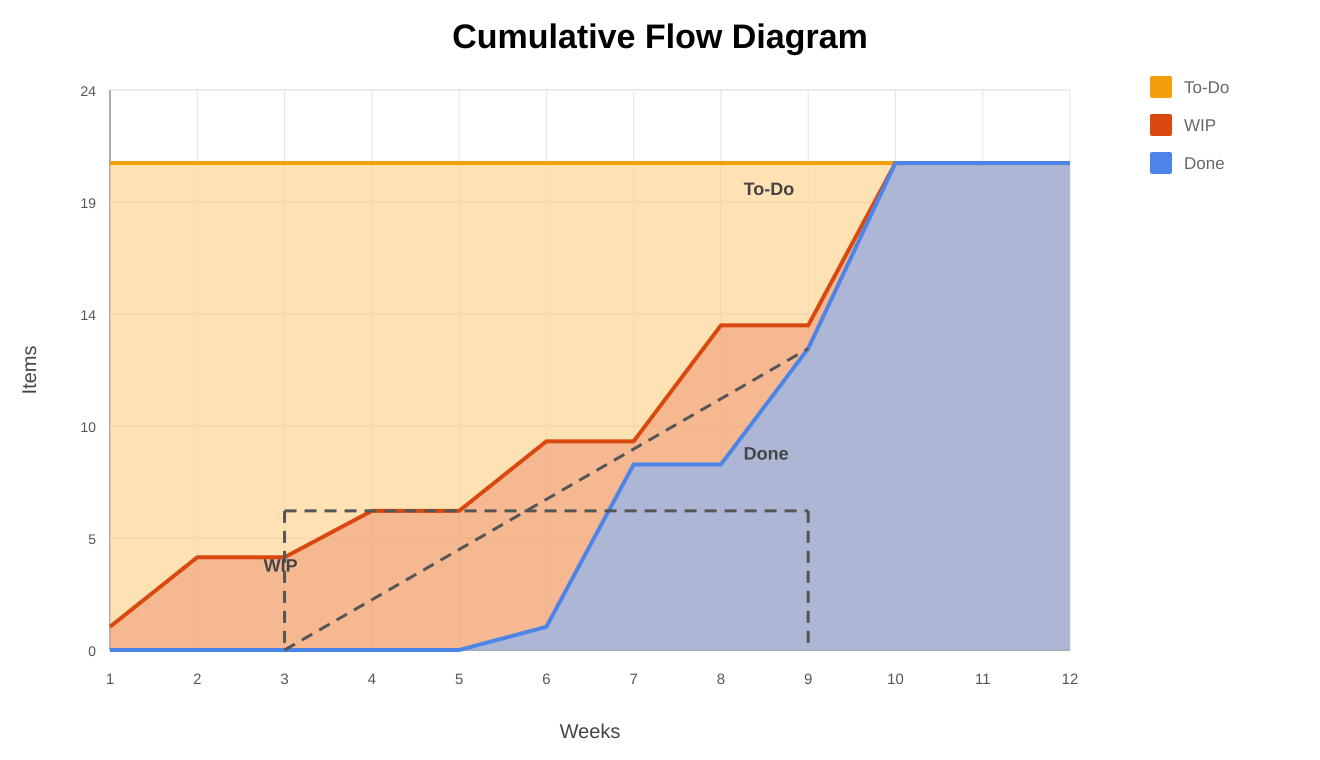
\includegraphics[width=\columnwidth]{figures/cfd.png}
\caption{Reconstructed cumulative flow across planned sprints.}
\label{fig:cfd}
\end{figure}

The CFD shows a healthy increase in completed work by the end of Sprint 4, but it also shows that a large amount of work remained open until Sprint 5. This matters because it explains the integration pressure visible at the end of March: the project behaved as a backend-first delivery, with many closing tasks landing close together.

\subsection{Throughput Report}
Two throughput lenses were used: sprint throughput measured as completed work items, and weekly implementation throughput measured as \texttt{feat:} commits in git.

\begin{figure}[htbp]
\centering
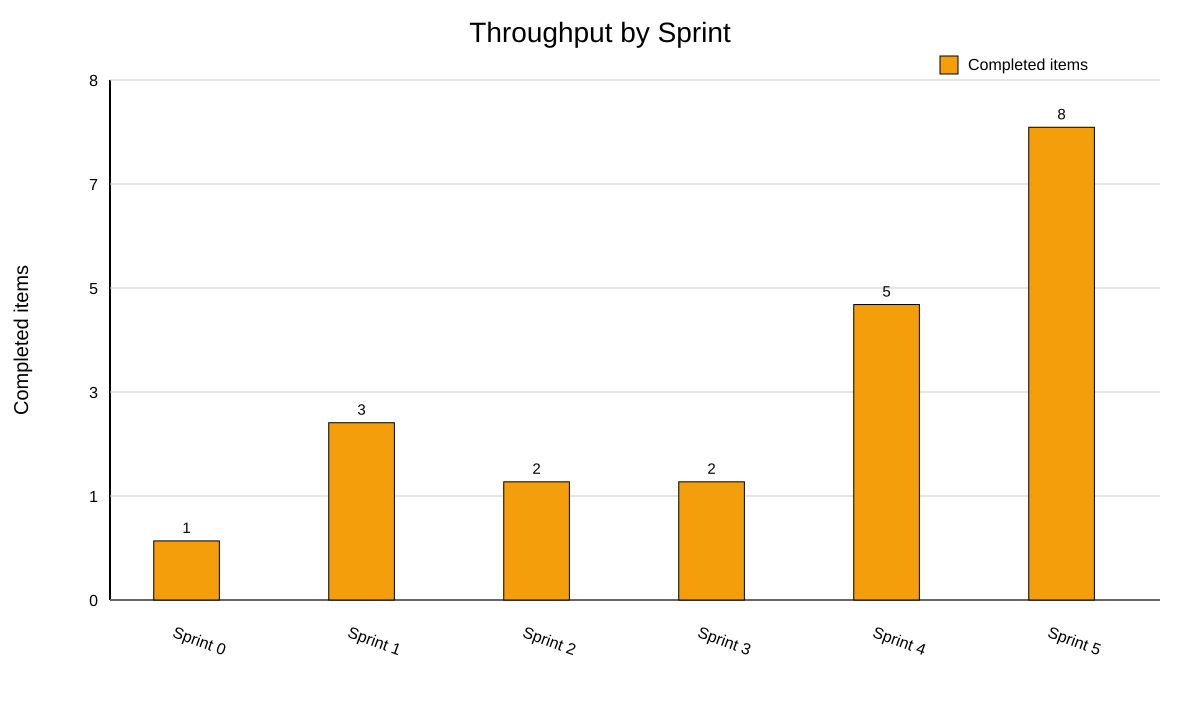
\includegraphics[width=\columnwidth]{figures/throughput.png}
\caption{Throughput by sprint based on completed backlog items.}
\label{fig:throughput}
\end{figure}

Sprint throughput rises from 3 items in Sprint 1 and 2 items in Sprint 2 and Sprint 3 to 5 items in Sprint 4 and 8 items in Sprint 5. This does not mean Sprint 5 was ``better managed'' than earlier sprints; rather, it indicates that integration-heavy and admin-heavy scope was compressed into the end of the backend cycle. That interpretation is consistent with the git history, where three active implementation weeks each contributed 7 feature commits.

\subsection{Sprint Burndown Chart}
The burndown was reconstructed across the full planned project timeline rather than only Sprint 5. Using the sprint windows defined in the SRS/README and the git-backed completion dates, we tracked cumulative planned scope and remaining work from Sprint 0 to Sprint 5.

\begin{figure}[htbp]
\centering
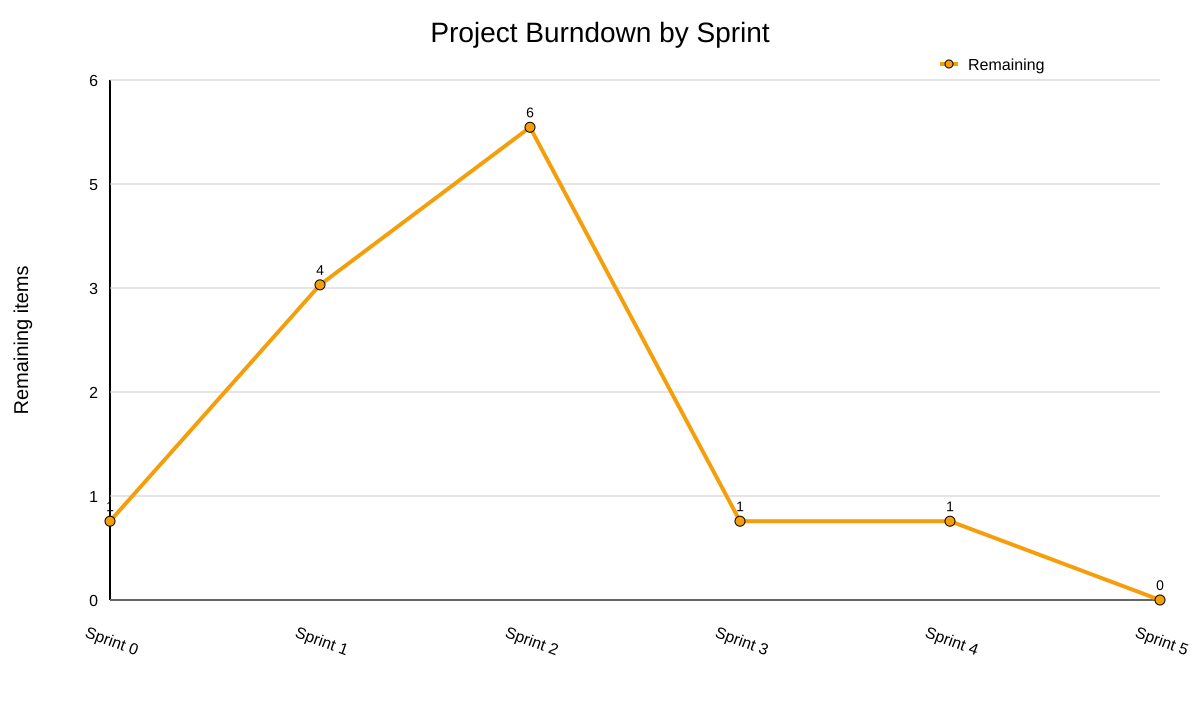
\includegraphics[width=\columnwidth]{figures/burndown.png}
\caption{Project burndown across Sprint 0 to Sprint 5.}
\label{fig:burndown}
\end{figure}

The resulting shape is revealing. Scope grows steadily from 1 tracked item in Sprint 0 to 21 cumulative items by Sprint 5, while completed work remains at 0 through Sprint 2, jumps sharply to 8 in Sprint 3, then 13 in Sprint 4, and closes at 21 in Sprint 5. This reflects how the repository history was actually committed: implementation landed in meaningful batches instead of continuously. That pattern is workable, but it increases the risk of hidden WIP and delayed integration feedback.

\subsection{Sprint Burnup Chart}
The corresponding burnup uses the same project-wide reconstruction. It compares cumulative completed work against cumulative planned scope at the end of each sprint.

\begin{figure}[htbp]
\centering
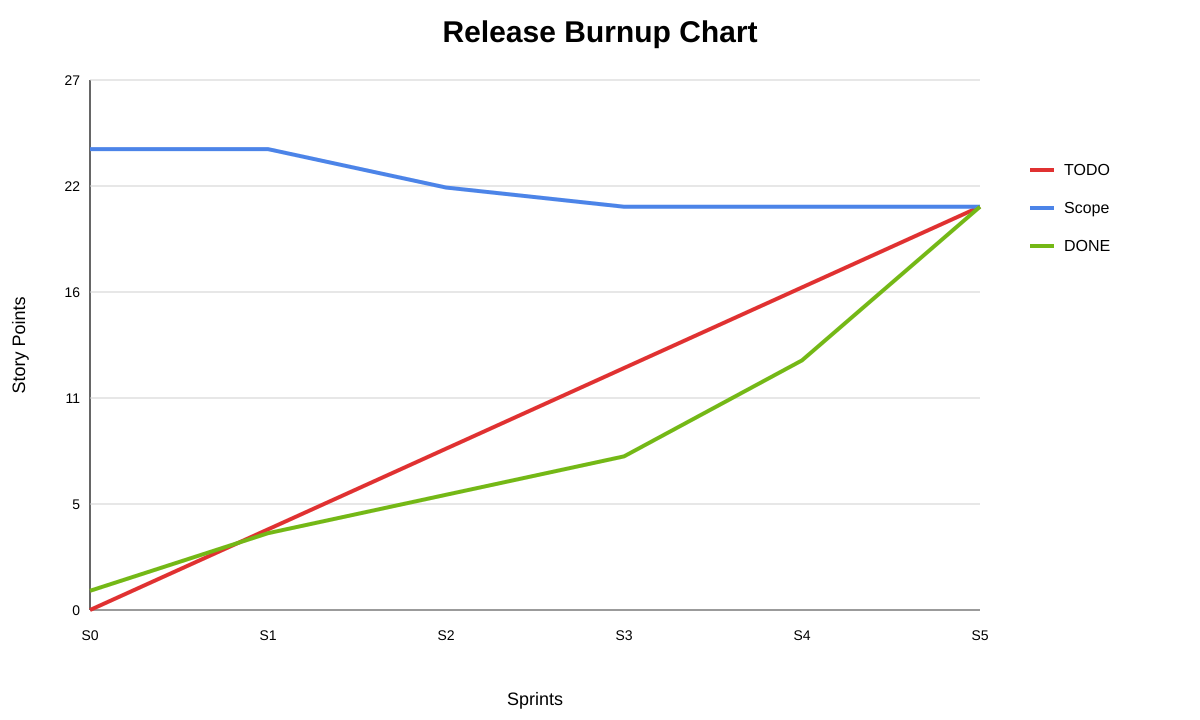
\includegraphics[width=\columnwidth]{figures/burnup.png}
\caption{Project burnup across Sprint 0 to Sprint 5.}
\label{fig:burnup}
\end{figure}

The burnup shows that project scope did not explode unexpectedly; instead, it expanded in a planned way as later sprints introduced appointments, billing, admin, notifications, and integration work. The more important observation is the lag between scope accumulation and completion. Sprint 3 and Sprint 5 each closed large chunks of the backlog, which suggests the team was capable of strong execution but tended to expose completion late.

\subsection{Additional Metric 1: Code Churn}
Code churn was computed from git \texttt{numstat} data aggregated by ISO week. It reflects development intensity and refactoring pressure.

\begin{figure}[htbp]
\centering
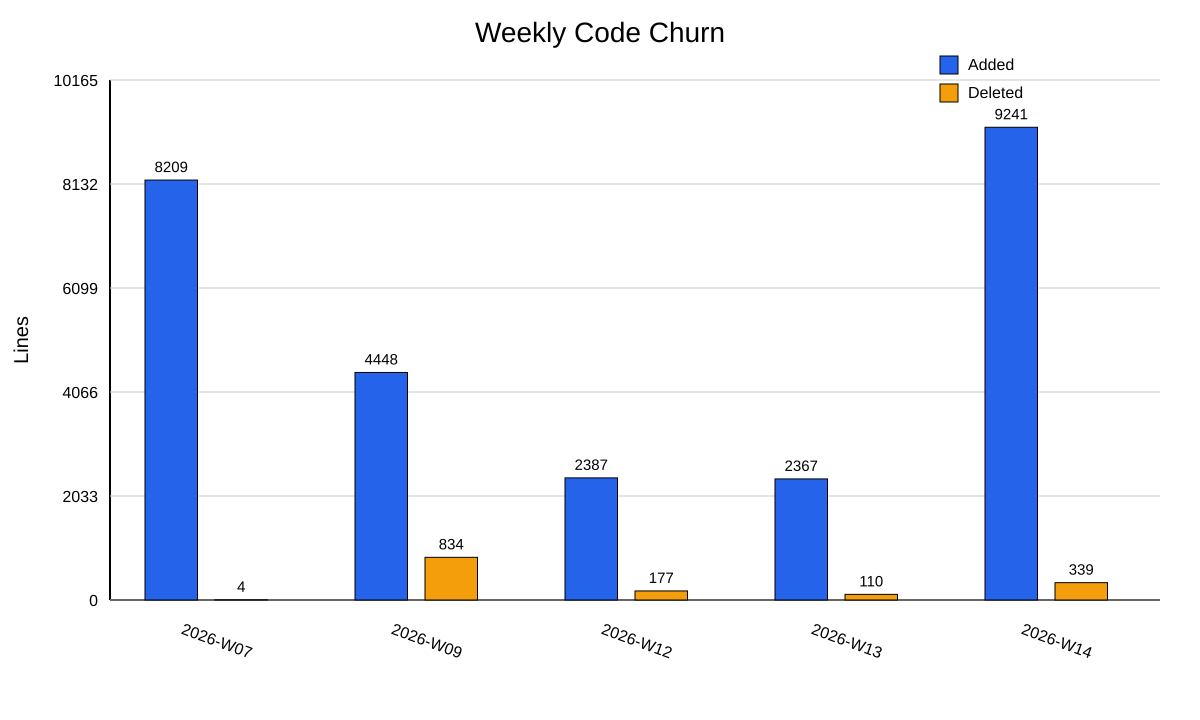
\includegraphics[width=\columnwidth]{figures/code_churn.png}
\caption{Weekly code churn from git history.}
\label{fig:churn}
\end{figure}

The highest churn appears in Week 07, when the repository moved from scaffolding to a usable backend foundation. Later weeks show smaller but still substantial additions, especially around Sprint 4 and Sprint 5. Importantly, deletion volume remains comparatively low, which suggests additive growth was still dominating over cleanup and consolidation.

\subsection{Additional Metric 2: Test Pass Rate and NFR Compliance}
The current \texttt{test\_cases.csv} contains 48 documented test cases and all 48 are marked PASS, giving a documented pass rate of \(100\%\). The response-time dataset also shows that every measured non-functional performance test remained within its target bound.

\begin{figure}[htbp]
\centering
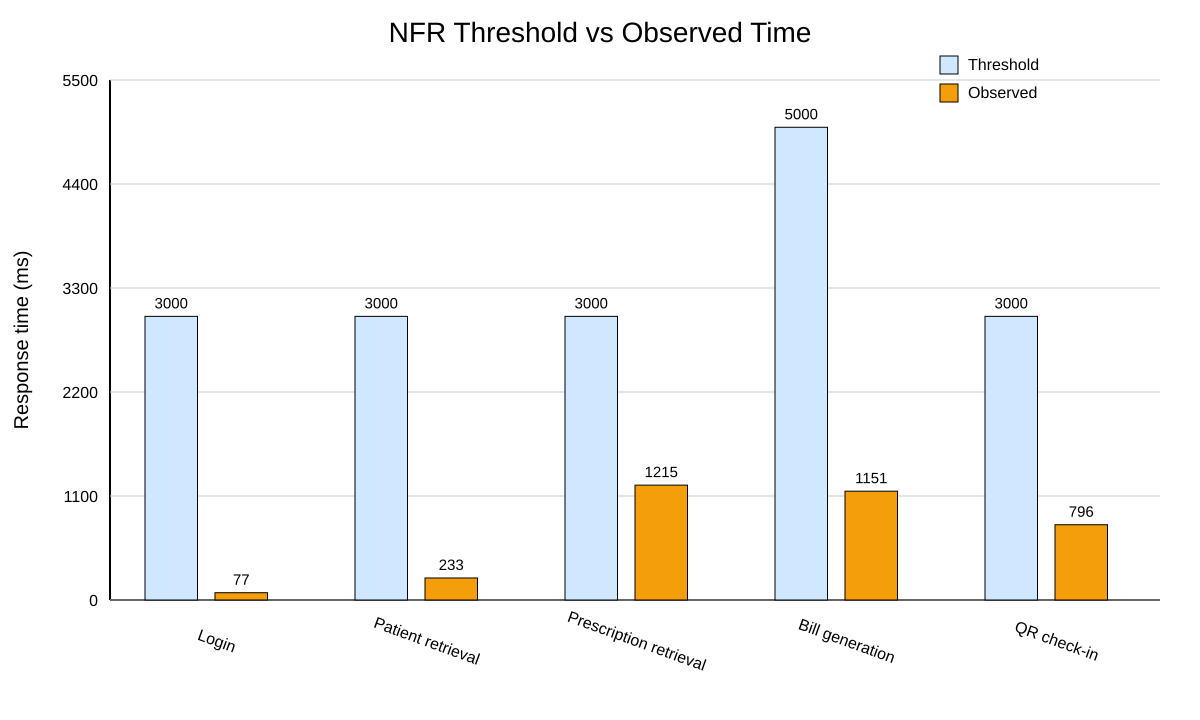
\includegraphics[width=\columnwidth]{figures/nfr.png}
\caption{Measured NFR timings versus target thresholds.}
\label{fig:nfr}
\end{figure}

The slowest documented operation was prescription retrieval at 1215\,ms, which still used only \(40.5\%\) of the allowed 3000\,ms threshold. Bill generation, despite being transactional, remained well below its 5000\,ms limit. The caveat is important: \texttt{smoke\_test.sh} now mentions 59 tests, whereas the checked-in CSV still records 48 cases. The project therefore has strong observed results but also a clear documentation-synchronization gap.

\section{Section II: Risk Assessment Matrix}
We rated each risk on a five-point probability scale and a five-point impact scale. Probability scores were assigned from repository evidence, sprint behavior, and project context rather than arbitrary intuition. Impact scores were based on expected effect on confidentiality, data integrity, schedule, or demonstrability. The risk score is \(P \times I\).

\begin{table*}[t]
\caption{Risk Assessment Matrix}
\centering
\footnotesize
\begin{tabular}{p{0.75cm} p{3.35cm} p{0.8cm} p{0.8cm} p{0.95cm} p{4.7cm} p{4.25cm}}
\hline
\rowcolor{HeaderBlue}
\textbf{ID} & \textbf{Risk} & \textbf{P} & \textbf{I} & \textbf{Score} & \textbf{Logic for Probability} & \textbf{Mitigation} \\
\hline
R1 & LDAP or authentication service instability blocks login and role validation. & 3 & 5 & 15 & The SRS depends on LDAP; authentication is a single-point gateway and was only fully hardened in late Sprint 5. & Keep Dockerized local LDAP, fail fast with clear 401/503 behavior, preserve seeded users, and verify auth in smoke/e2e runs before demos. \\
R2 & Database or migration failure corrupts clinical workflow continuity. & 3 & 5 & 15 & The project depends on Prisma Cloud plus evolving schema migrations, and most modules share visit-linked data. & Use Prisma migrations only, avoid destructive resets, keep seed idempotent, and verify \texttt{migrate deploy} during integration. \\
R3 & Cross-module integration regression breaks visit, lab, pharmacy, or billing flow. & 4 & 4 & 16 & The backend now spans 57 endpoints and 20 models; integration complexity is significantly higher than single-module risk. & Use transaction boundaries, end-to-end flow runner, smoke suite, and late-sprint API documentation review. \\
R4 & Documentation drift causes wrong test counts, stale setup steps, or submission mismatch. & 4 & 3 & 12 & This already appeared: README, smoke-test count, and CSV evidence were briefly out of sync. & Treat docs as sprint deliverables, update README/TESTING/CSV together, and regenerate assignment data from scripts. \\
R5 & Hidden work-in-progress causes late sprint compression and delivery risk. & 4 & 4 & 16 & Sprint 5 burn-down stayed flat until March 24 and then closed almost entirely in two days. & Break work into smaller verifiable items, force mid-sprint integration checkpoints, and track burn charts continuously rather than only at closeout. \\
R6 & Role-based access bug exposes medical data to unauthorized users. & 2 & 5 & 10 & PHC data is sensitive and the system has many role combinations, but route guards are consistently structured. & Keep \texttt{verifyJWT} and \texttt{authorizeRoles} mandatory, add RBAC tests, and review patient-only versus staff-only endpoints during Sprint 7. \\
R7 & Frontend lag creates a backend-complete but demo-incomplete product. & 4 & 3 & 12 & Sprint 6 had not started by April 3, 2026 while backend maturity had already increased substantially. & Freeze backend scope unless blocking, prioritize role dashboards, and reuse stable API contracts rather than changing backend routes mid-frontend sprint. \\
R8 & Performance hardening and deployment readiness remain weaker than functional readiness. & 2 & 4 & 8 & Response timings are good in lab conditions, but concurrency, HTTPS, and rate limiting are still scheduled for Sprint 7. & Preserve performance baselines, add load and security hardening later, and avoid presenting lab timings as production guarantees. \\
\hline
\end{tabular}
\label{tab:riskmatrix}
\end{table*}

The two highest-priority risks are R3 and R5. R3 is structural: once prescriptions, lab requests, billing, and notifications all depend on a shared visit model, regressions propagate quickly. R5 is process-driven: the charts show that integration happened in a compressed burst, which is efficient in the short term but fragile if repeated in Sprint 6 and Sprint 7.

\section{Section III: Mapping Risk Mitigation to the Sprint Plan}
The risk matrix is only useful if it changes the sprint backlog. Table \ref{tab:riskmap} shows how mitigations were already integrated into the implementation trajectory.

\begin{table*}[t]
\caption{Mapping Risks to Sprint Plan and Backlog}
\centering
\footnotesize
\begin{tabular}{p{1.0cm} p{3.2cm} p{4.7cm} p{6.3cm}}
\hline
\rowcolor{HeaderBlue}
\textbf{Sprint} & \textbf{Primary Risks Addressed} & \textbf{Backlog Response} & \textbf{Repository Evidence} \\
\hline
1 & R1, R2, R6 & Build authentication, JWT guards, schema foundation, and patient profile routes before any downstream module work. & \texttt{auth.routes.js}, \texttt{auth.service.js}, \texttt{auth.middleware.js}, Prisma schema alignment commits, patient profile routes. \\
2 & R2, R3, R6 & Stabilize the visit lifecycle and doctor attendance so later prescription, lab, and billing modules attach to a consistent workflow backbone. & Visit lifecycle endpoints, doctor availability and attendance modules, status transitions in services. \\
3 & R3, R6 & Add prescriptions and lab requests only after visit claiming and consultation existed; keep role-specific restrictions explicit. & Prescription and lab route files, role guards, lab upload audit trail, patient-access control extension. \\
4 & R2, R3, R8 & Use transactions for bill generation and QR check-in, and add operational modules without changing the central visit model. & Billing service with transaction logic, check-in service, medicine stock updates, document module, appointment constraints. \\
5 & R1, R3, R4, R5 & Add admin modules, notifications, end-to-end tests, API documentation, migrate-deploy verification, and real LDAP bind behavior. & Admin user management, reports, notifications, \texttt{e2e-full-flow.js}, \texttt{API\_DOCUMENTATION.md}, LDAP Docker setup, docs closeout commit. \\
6 & R5, R7 & Keep frontend scope focused on role dashboards, login flow, JWT storage, and route guards rather than adding fresh backend scope. The mitigation is to convert the stable Sprint 5 API surface into demonstrable UI slices role by role. & Sprint 6 plan in \texttt{README.md}: patient, doctor, reception, pharmacy, lab, and admin dashboards; login screen; JWT interceptor; role-based guards; logout and session expiry handling. \\
7 & R4, R6, R8 & Use the final sprint as a stabilization backlog rather than feature expansion. The mitigation is to gate release readiness on testing depth, RBAC verification, security hardening, performance checks, migration readiness, and demo preparation. & Sprint 7 plan in \texttt{README.md}: unit tests, integration tests, RBAC tests, security hardening, concurrent-load/performance check, final migration and seed validation, deployment plan, and final system demo preparation. \\
\hline
\end{tabular}
\label{tab:riskmap}
\end{table*}

This mapping shows that the team's sprint sequence was already acting as a risk-reduction strategy, exactly as proposed in the SRS. Foundations were delivered before workflow modules, workflow modules before operational extensions, and integration/hardening before the frontend. The main process lesson is that the Sprint 5 closeout should not become the norm: Sprint 6 needs more visible incremental closure.

\section{Conclusion}
The metric results support three clear conclusions. First, the PHC Integrated Digital System is already a non-trivial software product in backend terms: 57 endpoints, 20 domain models, about 2.9 KLOC of production logic, and an adjusted function-point count of 485.07. Second, the implementation quality is promising: all currently documented tests pass, measured response times remain comfortably below stated thresholds, and architecture is still disciplined enough that most logic sits in services instead of ad hoc controller code. Third, the biggest risks are no longer about raw implementation feasibility; they are about integration visibility, documentation synchronization, and frontend catch-up.

From a project-management standpoint, Sprint 5 succeeded functionally but exposed two operational weaknesses: work closed in a dense burst, and secondary artifacts did not always stay synchronized with the code. The immediate implication for the next phase is simple: Sprint 6 should prioritize visible dashboard delivery on top of the already-stable API, while Sprint 7 should emphasize RBAC testing, hardening, and deployment readiness.

\section*{AI Use Disclosure}
This report was prepared with assistance from AI-based tooling for language polishing, LaTeX drafting, and repository-driven metric scripting. All repository measurements, risk ratings, interpretations, and final content were manually reviewed against the project artifacts by the team before submission.

\section*{Progress Tracker Note}
As instructed in the lab handout, the detailed progression tracker can be shared separately as a private comment with the submission. The current team tracker is available at:
\newline
\href{https://docs.google.com/spreadsheets/d/1xLa2L8eWv8gfrIwPXrnImF8uManlRlRwRp3ksSOVI9E/edit?usp=sharing}{\texttt{Project tracker spreadsheet}}

\begin{thebibliography}{9}
\bibitem{boehm}
B. W. Boehm, \textit{Software Engineering Economics}. Englewood Cliffs, NJ, USA: Prentice-Hall, 1981.

\bibitem{halstead}
M. H. Halstead, \textit{Elements of Software Science}. New York, NY, USA: Elsevier, 1977.

\bibitem{albrecht}
A. J. Albrecht and J. E. Gaffney, ``Software Function, Source Lines of Code, and Development Effort Prediction: A Software Science Validation,'' \textit{IEEE Transactions on Software Engineering}, vol. SE-9, no. 6, pp. 639--648, Nov. 1983.

\bibitem{scrum}
K. Schwaber and J. Sutherland, \textit{The Scrum Guide: The Definitive Guide to Scrum}, 2020.

\bibitem{ieee830}
IEEE, \textit{IEEE Recommended Practice for Software Requirements Specifications}, IEEE Std 830-1998, 1998.

\bibitem{srs}
Team PHC Integrated Digital System, \textit{Software Requirements Specification Version 2.0}, IIT Jodhpur, Feb. 4, 2026.

\bibitem{repo}
PHC Integrated Digital System Repository Artifacts: \texttt{README.md}, \texttt{TESTING.md}, \texttt{test\_cases.csv}, \texttt{backend/prisma/schema.prisma}, route and service files, and git history accessed Apr. 3, 2026.
\end{thebibliography}

\end{document}
